\section{Concept of the method} % 2 pages
\label{sec:concept}

If a small signal sits on
a large background, relatively small changes to the background shape can
have significant effects on the apparent signal size and position.
Unless there is a
reliable theory or simulation which can constrain the background shape,
there is an uncertainty about which function to use to fit
the background. Hence, different choices of the form of the function
will give different results for the signal parameters, meaning there is a
systematic uncertainty associated with the choice of function.
The basic concept discussed in this paper is to consider this choice 
as a source of systematic error which is modelled as a nuisance parameter.
It is then consistently treated like other nuisance parameters as far as
possible.

The two main parameters of a signal are the position (i.e. the mean)
and size (i.e. the amplitude), although other
quantities such as the width may also be of interest. This results in a
multi-dimensional parameter space. For simplicity in this paper, the position
and width of the signal are considered to be known and only the signal
size is to be determined. However, the method is also applicable to
cases where more than one parameter is being estimated.

\subsection{Continuous nuisance parameters}
\label{sec:concept:continuous}

It is useful to consider briefly the usual way in which nuisance 
parameters are used to incorporate systematic errors. Consider measuring a signal
property for a known background functional shape, but with unknown function
parameters. The background parameters themselves are considered as
nuisance parameters, since their actual values are not of interest.
When fitting for a parameter of interest $x$, then twice the negative logarithm of the
likelihood (\nll) is minimised with respect to $x$ and all the
nuisance parameters. It is usual to construct a profile likelihood
such that \nll is minimised with respect to the nuisance parameters 
for each value of $x$ over a range. 
The (for example) 68.3\% confidence interval of $x$ 
is then
taken as the region for which \nll is less than ${\rm \nll}_{BF}+1$,
where ${\rm \nll}_{BF}$ is the best-fit value at the overall minimum. 
Similarly, the 38.3\%, 95.4\% and 99.7\% confidence intervals are defined by the 
regions in which \nll is less than ${\rm \nll}_{BF}+0.25$, ${\rm \nll}_{BF}+4$ 
and ${\rm \nll}_{BF}+9$, respectively. 

Consider this absolute minimum in \nll: if the nuisance parameters at that
point were fixed, then the profile \nll curve would be steeper than for
the original overall \nll curve. This directly reflects the fact that
if the nuisance parameters had no uncertainty,
the error on $x$ would be reduced, i.e. there would be no systematic 
uncertainty arising from this source.
The same is true for any other point on the original curve; if the nuisance
parameters were not allowed to vary, each would result in a new steeper curve,
in these cases with a minimum above the original curve.
The width of these curves would again only be affected by the statistical
power of the dataset being fitted, not by the systematic errors encompassed
in the nuisance parameters.
Finally, there are in general
many other sets of nuisance parameters which do not result in a point on the
original profile curve. Fixing the parameters to these values will also result
in further curves which are enclosed by the original profile curve.
The critical point is that the overall minimum as a function
of $x$ encloses the curves for all possible values of the nuisance
parameters.

Now consider finding the profile curve in a different way, illustrated
in figure~\ref{fig:concept:cartoon}.
Each set of nuisance
parameter values will result in a curve, the steepness of which reflects 
the statistical error only. Consider picking many different sets of nuisance
parameter values; each gives one such curve. Drawing an ``envelope'' around the
minimum \nll value of all these curves will give an approximation to the
original profile curve. Clearly, in practice, many such sets of nuisance
parameter values would be needed to make this curve smooth. However, in
principle, sampling the nuisance parameter space sufficiently
and then finding the enclosing
minimum envelope should give the profile curve required.
Note, it would of course be possible to mix the two methods, i.e.
choose sets of only some of the parameter values and fit for the others.
%
\begin{figure}[tbp]
\centering
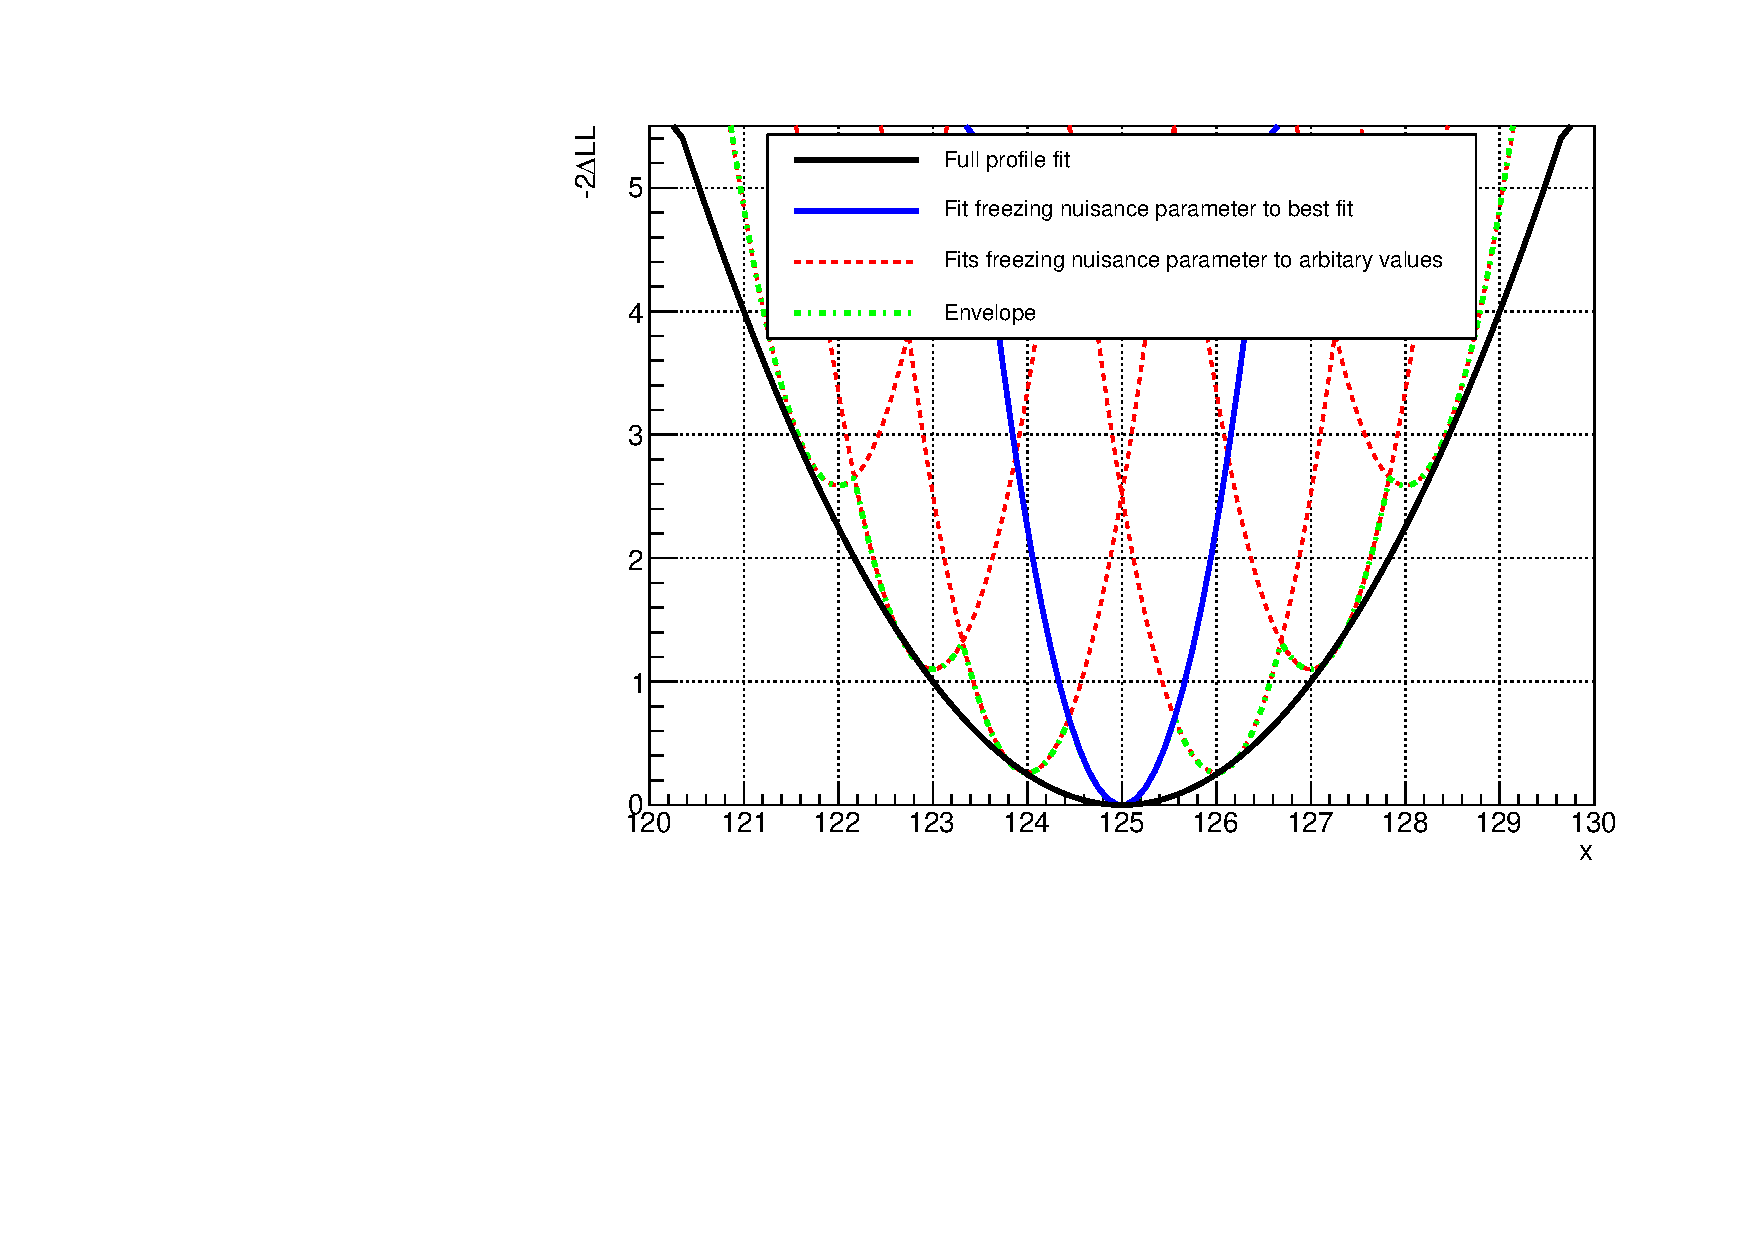
\includegraphics[width=0.6\textwidth]{concept/envelope_cartoon.pdf}
\caption{Illustration of construction of the envelope (green, dot-dashed line)
by choosing several fixed values of the nuisance parameters (red, dashed lines)
when performing a profile likelihood scan for a variable of interest $x$.
The \nll profile curve for the nuisance parameters fixed to the best fit
values is shown by the blue, solid line. The full profile curve allowing the
nuisance parameters to be fitted for every value of $x$ is shown by the 
black, solid line. The red dashed lines show the \nll curves for fixed 
nuisance parameter values other than those at the best fit, while the green 
dashed line is the envelope, i.e. the lowest value of any of the red dashed 
curves for each $x$. Even with such a coarse sampling of the nuisance 
parameters, it is seen that the envelope approximates the full profile curve.}
\label{fig:concept:cartoon}
\end{figure}

\subsection{Background function uncertainty}
\label{sec:concept:functions}

The method of picking various sets of nuisance parameters and finding
an envelope can conceptually be applied to the uncertainty on the background functional form. 
Each background function considered can be labelled by an
integer. The integer is then treated as a (discrete) nuisance parameter
for the profile calculation and hence this method has been termed
``discrete profiling''.
The minimum envelope then gives the overall profile curve including
all functions considered. This automatically includes any systematic error
arising from the choice of function, as the envelope will in general be broader
than any of the individual curves which contribute to the envelope.

In practical terms, most minimisation routines 
cannot easily handle a discrete parameter, particularly when the
number and values of the other parameters of the fit (i.e. the parameters
of the functions) change with the discrete parameter.
Hence, in practice it has
to be handled by mixing the methods as discussed in the previous section,
i.e. choose each function and minimise
the other parameters in the usual way to give a profile curve for each function
in turn. 

While the concept is straightforward, there are some statistical
issues in applying it.
Firstly, there is a question of whether the \nll minimum envelope covers,
i.e. has the correct properties for a profile curve.
This is discussed in Section~\ref{sec:functions}.
Secondly, to find the minimum requires a
comparison between the absolute \nll values from fits to different functions.
In general, these will include functions with different numbers of parameters.
Hence, a way to meaningfully compare their \nll values must be found.
This is discussed in Section~\ref{sec:correction}.
